\chapter{Reinforcement Learning}

Reinforcement learning (RL) \cite{Sutton1998} is all about the interaction between an agent and its environment. Learning occurs through trial-and-error, where the agent observes the state of the environment, takes actions based on these observations, influences new possible state configurations, and perceives rewards based on its previous decisions. The entire sequence of decisions is directed towards achieving a goal, such as escaping from a maze, \href{https://arxiv.org/abs/1312.5602}{winning an Atari Game} \citep{mnih2013playing}, or \href{https://deepmind.google/technologies/alphago/}{defeating the world champion of Go} \citep{silver2016mastering}. How does the agent learn to act to achieve its goal? RL algorithms are designed to maximize the total rewards obtained by the agent, thus guiding its actions towards achieving its objectives. \\

\noindent In this chapter, we will introduce RL with the essential concepts required for implementing these agents. Specifically, we will focus on model-free RL, where the agent does not aim to understand the underlying model of its environment (unlike model-based RL). Instead, the goal is to design agents that learn to perform well solely by consuming experiences from their environment. By understanding the basics of designing such agents, we will explore policy optimization methods used to learn the agent’s behavior. We will then take a step further to build agents on top of diffusion models that learn how to generate better samples aligned with the goals specified by a reward model.

\section{The Framework for Learning to Act}

The starting point for designing agents that learn to act is the Markov Decision Process (MDP) framework \cite{Sutton1998}. An MDP is a mathematical object that describes the interaction between the agent and the environment. This interaction is characterized by a tuple $\langle \mathcal{S}, \mathcal{A}, P, R, \rho_{0}, \gamma \rangle$, where:

\begin{enumerate}
    \item $\mathcal{S}$, \textbf{state space}, set of possible states in the environment.
    \item $\mathcal{A}$, \textbf{action space}, set of possible actions available to the agent.
    \item $P: \mathcal{S}\times\mathcal{A}\rightarrow\Delta(\mathcal{S})$, \textbf{transition probability distribution}, which gives the probability
    of the environment for transitioning to a new state $s_{t+1}$ with a reward $r_t$ given the current state $s_{t}$ and action $a_{t}$.
    \item $R: \mathcal{S}\times\mathcal{A}\rightarrow\mathbb{R}$, 
    \textbf{reward function}, which provides a scalar feedback signal $r_{t}$ (aka reward) $r_{t}$ to the agent after taking an action $a_{t}$ and reaching the subsequent state $s_{t+1}$.
    \item $\rho_{0}$, \textbf{initial state distribution}, which determines the probability of the agent starting in a particular state.
    \item $\gamma\in\left[0, 1 \right]$ is the \textbf{discount factor}, which determines the importance of future rewards.
\end{enumerate}

\begin{figure}[ht]
    \centering
    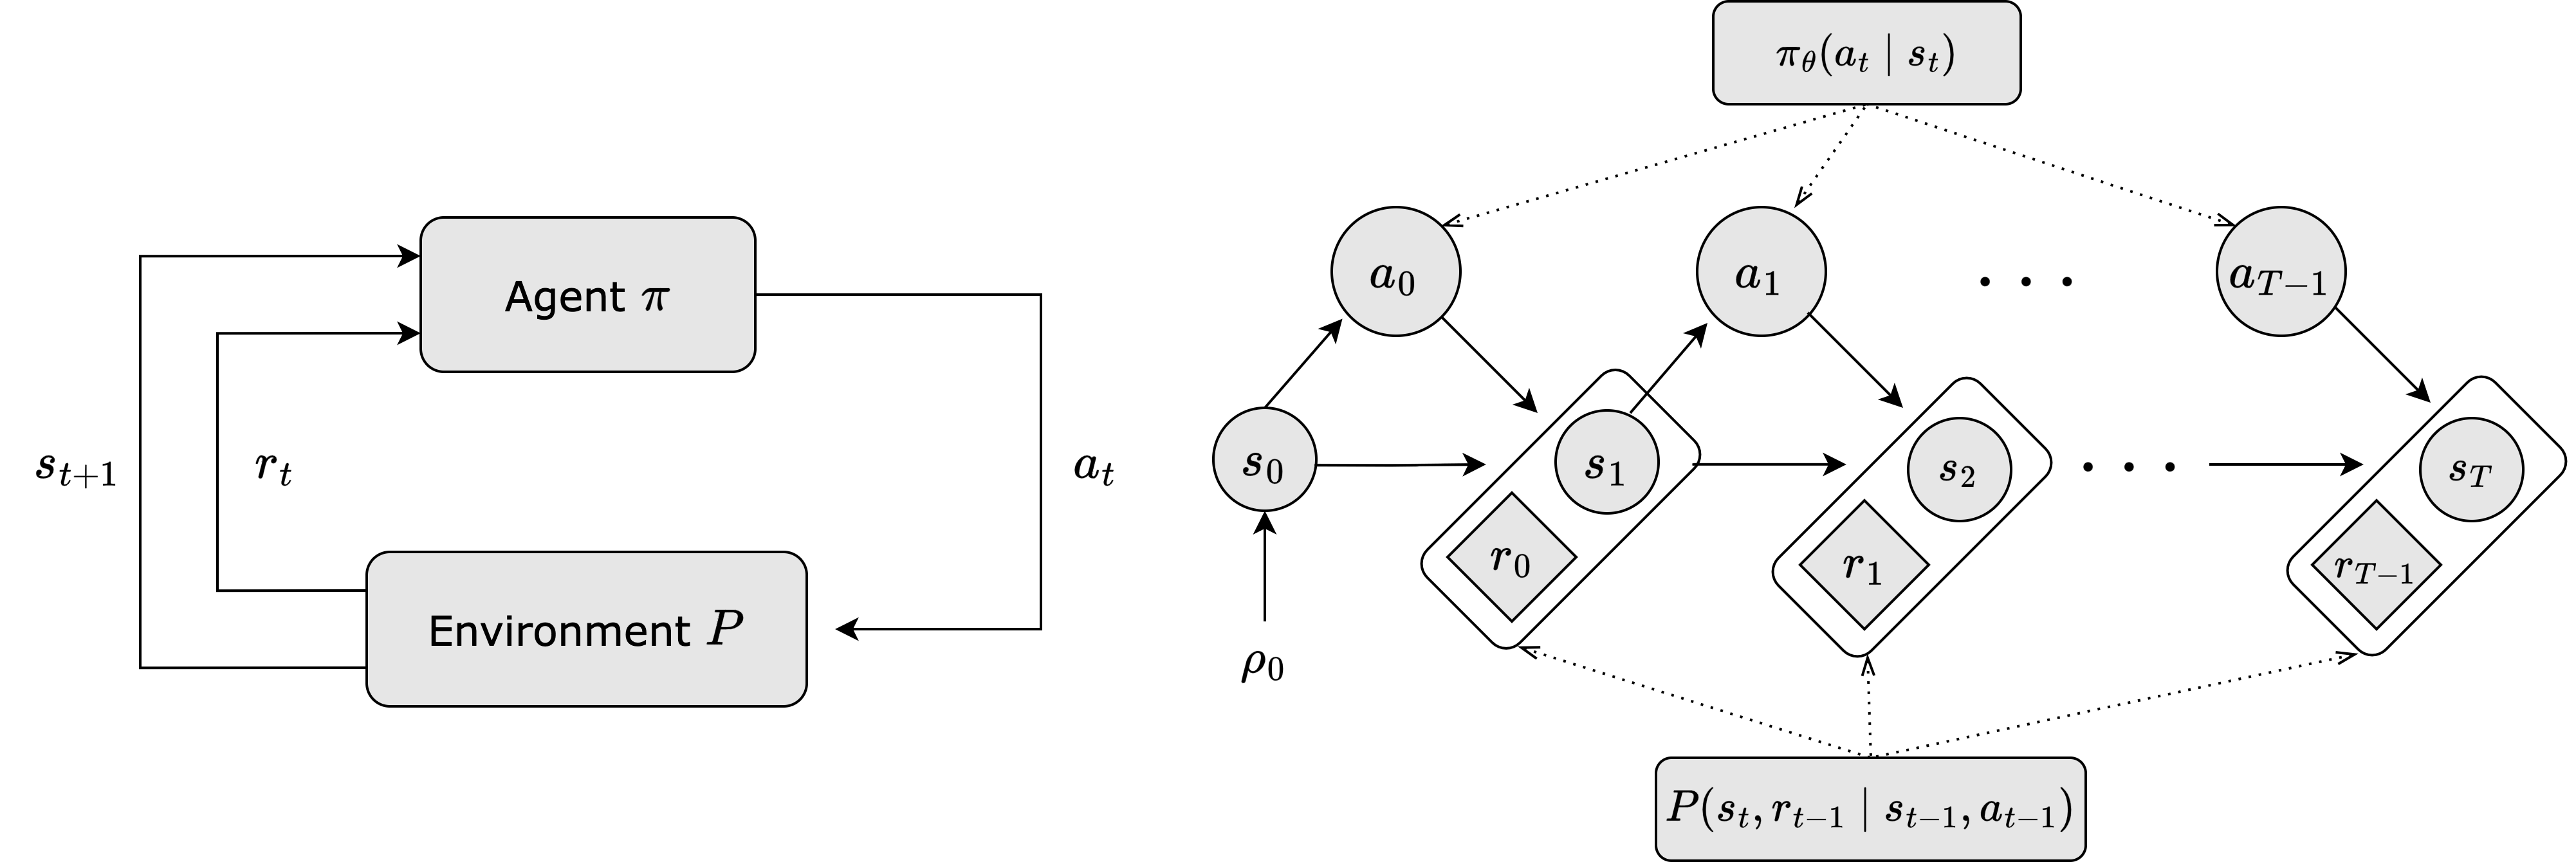
\includegraphics[scale=0.63]{ch3-rl/MDP-diagram.png}
    \captionsetup{width=\textwidth} % set the width of the caption
    \caption{\textbf{Left:} A loop representation of a Markov Decision Process (MDP). \textbf{Right:} An unrolled MDP depecting an episodic case with a finite horizon $T$ and a parameterized policy $\pi_{\theta}$.}
    \label{fig:mdp-diagram}
  \end{figure}


\noindent MDPs generate sequences of state-action pairs, or trajectories $\tau$, starting from an initial state $s_{0}\sim\rho_{0}$. The agent's behavior is determined by a policy $\pi:\mathcal{S}\rightarrow\Delta(\mathcal{A})$, which maps states to a distribution over actions. An action $a_{0}\sim\pi(s_{0})$ is selected, leading to the next state $s_{1}$ from transition distribution and a reward $r_{0}=R(a_{0}, s_{0})$. This process repeats iteratively, with the agent selecting actions, transitioning through states, and receiving rewards (see left side of Figure~\ref{fig:mdp-diagram}). \\

\noindent The process can run indefinitely, known as an infinite horizon, or be confined to episodes with terminal states, referred to as episodic tasks, such as winning or losing a game (see the right side of Figure~\ref{fig:mdp-diagram}). Notice that the transition depends only on the current state and action, not on the sequence of events that preceded it. This is the \textit{Markovian property}, which states that the future and the past are conditionally independent, given the present (\textit{memoryless}). In this work, we will focus on the episodic setting. \\

\noindent In reinforcement learning, the main purpose is for the agent to develop a policy $\pi$ that maximizes the expected return ($R$) for each episode. \\

\begin{equation*}
    \underset{\pi}{\text{maximize }} \mathbb{E}_{\tau\sim\pi}\left[R(\tau)\right]
\end{equation*}

\noindent The return over a trajectory $\tau$ is defined as the accumulated discounted rewards of the trajectory, $R(\tau) = \sum_{t=0}^{T-1}\gamma^{t}r_{t}$. The reward signals $r_{t}$ are the inmmediate effect of taking the actions, and the return is the cumulative rewards obtained during the trajectory, considering a discount factor $\gamma$, which gives more importance to the rewards of nearer actions than to future rewards. 


\section{Policy Optimization}

In reinforcement learning there a different approaches to solve the MDP formulated in the previous section (Figure~\ref{fig:rl-model-free-taxonomy}). The most common are value-based methods and policy-based methods. In value-based methods, the agent learns which state is more valuable and
take action that leads to it.
% a \textit{value function} ($V^{\pi}(s_{t})$) a measure goodnes of states or state-action pairs, i.e., an estimate of the expected value of a given state. 
In policy-based methods, the agent learns a policy that directly maps states to actions. This work we will focus on the last methods, specifically in policy gradients. \\

\begin{figure}[ht]
    \centering
    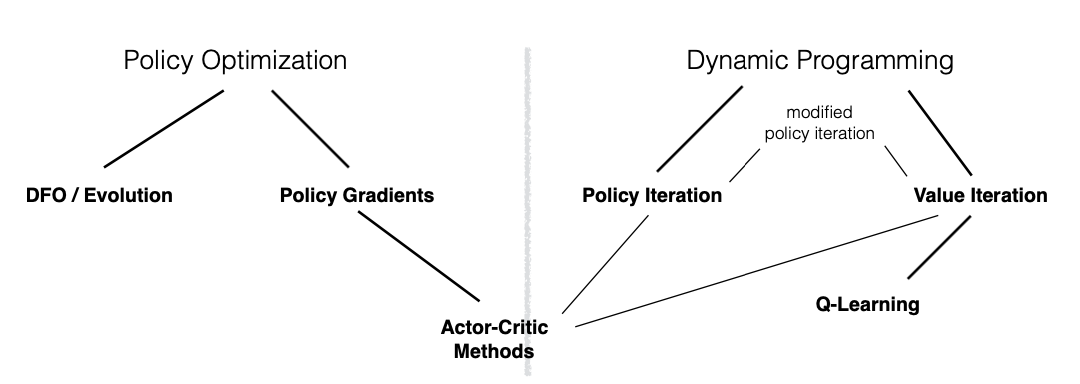
\includegraphics[scale=0.80]{ch3-rl/rf-solve-methods-schulman-thesis-img.png}
    \captionsetup{width=\textwidth} % set the width of the caption
    \caption{Illustration of a taxonomy of model-free RL algorithms. \textbf{Source:} \href{https://rail.eecs.berkeley.edu/deeprlcourse/}{Optimizing Expectations: From Deep Reinforcement Learning to Stochastic Coomputation Graphs} by John, Schulman (2016) \cite{schulman2016optimizing}.}
    \label{fig:rl-model-free-taxonomy}
  \end{figure}

\noindent Other approaches for finding a policy is by non solving the MDP, 
but by directly optimizing the policy. This is the case of derivative free
optimization (DFO), or evolutionary algorithms, in which the policy is parameterized by a vector $\theta$, and the agent explores the space of parameters by searching. Nothing of the temporal structure and actions of the MDPs are considered in this kind of solution. \\

% Tesis de Schulman final capítulo 4 GAE
\noindent Policy gradient methods provide a way to reduce reinforcement learning to stochastic gradient descent, by providing a connection between
how function approximation is solved in supervised learning settings.

\subsection{Learning the Policy}

The starting point is to think of trajectories as units of learning instead of individual observations (i.e., actions). What dynamics generate a trajectory? 
Given a policy $\pi_{\theta}$, represented as a function with parameter $\theta\in \mathbb{R}^{d}$, whose input is a representation of the state and whose output is action selection probabilities, we can deploy the agent into its environment at an initial state $s_0$ and observe its actions in inference mode or \textit{evaluation phase} \citep{sutton1999policy}. The agent continuously promotes actions based on the current state $s_{t}$ until the episode ends in a terminal state, when $t=T$. At this point, we can determine if the goal was accomplished, such as winning the ATARI Pong game, \textit{or generating aesthetically pleasing samples from a diffusion model}. 
% The reward signals are the inmmediate effect of taking the actions, and the returns are the cumulative rewards obtained during the trajectory. 
The returns are the scalar value that assets perfomance whether we have achieved the ultimate goal, effectively acting as a ``proxy'' of a label for the overall trajectory. Thus, the trajectory serves as our unit of learning, and the remaining task is to establish the feedback mechanism for the \textit{learning phase}. \\

\noindent Intuitivelly, we want to collect the trajectories and make the good trajectories and actions more probable, and push the actions towards betters actions. \\

\noindent Mathematically, we aim to perform stochastic optimization to learn the agent’s parameters. This involves obtaining gradient information from sample trajectories, with performance assessed by a scalar-value function (i.e., reward). The optimization is stochastic because both the agent and the environment contain elements of randomness, meaning we can only compute estimates of the gradient. Crucially, we are estimating the gradient of the expected return with respect to the policy parameters. To address this, we employ Monte Carlo Gradient Estimation \citep{mohamed2020monte}, specifically using the score function method. From a machine learning perspective, this involves dealing with the stochasticity of the gradient estimates, $\hat{g}$, and using gradient ascent algorithms to update the policy parameters based on these estimates, along with a learning rate $\alpha$ to control the step size of the optimization process.

\begin{equation}\label{eqn:gradient-ascent}
    \theta \leftarrow \theta + \alpha \hat{g}_{N}
\end{equation}


\subsection{Gradient Estimation via Score Function}\label{sec:gradient-estimation-score-function}

The gradient estimation can be obtained using the score function gradient estimator. Let's introduce the following probability objective $\mathcal{F}$, defined in the \href{https://en.wikipedia.org/wiki/Ambient_space_(mathematics)}{ambient space} $\mathcal{X}\in\mathbb{R}^n$ and with parameters $\theta\in\mathbb{R}^n$,

\begin{equation}\label{eqn:probability-objective}
\mathcal{F}(\theta) = \int_{\mathcal{X}} p(\mathrm{x; \theta})f(\mathrm{x})~d\mathrm{x} = \mathbb{E}_{p(\mathrm{x};\theta)}\big[f(\mathrm{x})\big]
\end{equation}

\noindent Here, $f$ is a scalar-valued function, similar to how the reward is represented in the reinforcement learning setting. The \textit{score function} is the derivative of the log probability distribution $\nabla_{\theta}\log p(\mathrm{x};\theta)$ with respect to its parameters $\theta$. We
can use the following identity to establish a connection between
the score function and the probability distribution $p(\mathrm{x};\theta)$.

\begin{equation}\label{eqn:log-derivative-trick-expression}
    \begin{split}
        \nabla_\theta\log p(\mathrm{x};\theta) &= \frac{\nabla_{\theta}p(\mathrm{x}; \theta)}{p(\mathrm{x};\theta)} \\
        p(\mathrm{x};\theta) \nabla_{\theta}\log p(\mathrm{x};\theta) &= \nabla_{\theta}p(\mathrm{x};\theta)
    \end{split}
\end{equation}

\noindent Therefore, taking the gradient of the objective $\mathcal{F}(\theta)$ with respect to the the parameter $\theta$, we have

\begin{equation}\label{eqn:score-function-gradient-objective}
    \begin{split}
        g = \nabla_{\theta} \mathbb{E}_{p(\mathrm{x};\theta)}[f(\mathrm{x})] &= \nabla_{\theta}\int_{\mathcal{X}} p(\mathrm{x};\theta) f(\mathrm{x}) d\mathrm{x} \\
        &= \int_\mathcal{X} \nabla_{\theta}~p(\mathrm{x}; \theta)f(\mathrm{x})d\mathrm{x} \\
        &= \int_{\mathcal{X}}p(\mathrm{x};\theta)\nabla_{\theta}\log p(\mathrm{x}; \theta) f(\mathrm{x})d\mathrm{x} \\
        &=\mathbb{E}_{p(\mathrm{x};\theta)}\big[f(\mathrm{x})\nabla_{\theta}\log p(\mathrm{x};\theta) \big] 
    \end{split}
\end{equation}

\noindent The use of the log-derivative rule of Equation~\ref{eqn:log-derivative-trick-expression} to introduce the score function in Equation~\ref{eqn:score-function-gradient-objective} is also known as the \href{https://blog.shakirm.com/2015/11/machine-learning-trick-of-the-day-5-log-derivative-trick/}{\textit{log-derivative trick}}. Now, we can compute an estimate of the gradient, $\hat{g}$, using Monte Carlo estimation with samples from the distribution $p(\mathrm{x};\theta)$ as follows:

\begin{equation}\label{eqn:score-function-gradient-estimator}
    \hat{g}_{N} = \frac{1}{N}\sum_{i=1}^{N}f\big(\hat{\mathrm{x}}^{(i)}\big) \nabla_{\theta}\log p\big(\hat{\mathrm{x}}^{(i)};\theta\big)
\end{equation}

\noindent We draw $N$ samples $\hat{\mathrm{x}}\sim p(\mathrm{x};\theta)$, compute the gradient of the log-probability for each sample, and multiply by the scalar-valued function $f$ evaluated at the sample. The average of these terms is an unbiased estimate of the gradient of the objective $g$, which we can use for gradient ascent using Equation~\ref{eqn:gradient-ascent}.

% , along with a learning rate $\alpha$ to control the step size of the optimization process. The update rule for the parameter $\theta$ is as follows:

\noindent There are two important points to mention about Equation~\ref{eqn:score-function-gradient-estimator}.

\begin{enumerate}
    \item The function $f$ can be any arbitrary function we can evaluate on $\mathrm{x}$. Even if $f$ is nondifferentiable with respect to $\theta$, it can still be used to compute the gradient estimation $\hat{g}$.
    \item The expectation of the score function is zero, meaning that the gradient estimator is unbiased.
    \begin{equation}\label{eqn:score-function-expectation-zero}
    \begin{split}
        \mathbb{E}_{p(\mathrm{x};\theta)}\big[\nabla_{\theta}\log p(\mathrm{x};\theta)\big] 
        &= \int_{\mathcal{X}}p(\mathrm{x};\theta)\nabla_{\theta}\log p(\mathrm{x}; \theta) d\mathrm{x} \\
        &= \int_{\mathcal{X}} p(\mathrm{x};\theta)\frac{\nabla_{\theta} p(\mathrm{x}; \theta)}{p(\mathrm{x};\theta)}d\mathrm{x} \\
        &= \int_{\mathcal{X}}\nabla_{\theta}p(\mathrm{x};\theta)d\mathrm{x} \\
        &= \nabla_{\theta}\int_{\mathcal{X}} p(\mathrm{x}; \theta)d\mathrm{x} = \nabla_{\theta} 1 =0
    \end{split}
    \end{equation}
\end{enumerate}

\noindent The last point is particularly useful because we can replace $f$ with a shifted version given a constant $\beta$, and still obtain an unbiased estimate of the gradient, which can be beneficial for the optimization task.

\begin{equation}\label{eqn:score-function-gradient-estimator-baseline}
\hat{g}_{N} = \mathbb{E}_{p(\mathrm{x}_{\theta})}\big[(f(\mathrm{x}) - \beta) \nabla_{\theta} \log p(\mathrm{x}; \theta)\big]
\end{equation}

\noindent Using a \textbf{\textit{baseline function}} to determine $\beta$, that does not depend on the parameter $\theta$, can reduce the variance of the 
estimator \citep{mohamed2020monte}. The baseline function, which satisfies the property in Equation~\ref{eqn:score-function-expectation-zero}, can be any function independent of
$\theta$. When a baseline is chosen to be close to the scalar-valued function $f$, it effectively reduces the variance of the estimator. This reduction in variance helps stabilize the updates by minimizing fluctuations in the gradients estimates, leading to more reliable and efficient learning.

\section{Vanilla Policy Gradient, aka REINFORCE}\label{sec:reinforce}

The REINFORCE algorithm \citep{williams1992simple} translates the previous 
derivation of gradient estimation via the score function into reinforcement learning terminology. This is the earliest member of the Policy Gradient family (Figure~\ref{fig:rl-model-free-taxonomy}), where the objective is to maximize the expected return of the trajectory $\tau$ under a policy $\pi$ parameterized by $\theta$ (e.g., a neural network). At each state $s_{t}$, the agent takes an action $a_{t}$ according to the policy $\pi$, which generates a probability distribution over actions $\pi(a_{t}\mid s_{t};\theta)$. Here, we will use the notation $\pi_{\theta}(\cdot)$ instead of $\pi(\cdot;\theta)$. \\

\noindent As we mentioned in previous section, a trajectory $\tau$ represents the sequence of state-action pairs resulting from the agent's interaction with its environment. From the initial state $s_{0}$ to the terminal state $s_{T}$, the trajectory $\tau$ is a sequence of states and actions, $\tau = (s_{0}, a_{0}, \dots, s_{T-1}, a_{T-1}, s_{T})$, which describes how the agent
acts during the episodic task. Let $p_{\theta}(\tau)$ be the
probability of obtaining the trajectory $\{\tau^{(i)}\}_{0:T}$ under the policy $\pi_{\theta}$. \\

\noindent We thus have a distribution of trajectories. Recall that the unit of learning is the trajectory $\tau$, and the goal is to maximize the expected return of the trajectory. The return $R(\tau)$ could be the cumulative rewards obtained during the \textit{episode} or the discounted rewards. The expected return is given by the following expression:

\begin{equation}\label{eqn:rl-objective}
    \mathcal{J}(\theta)=\mathbb{E}_{\tau\sim p_{\theta}(\tau)}[R(\tau)] 
\end{equation}

\noindent This is the objective we want to maximize, which is a 
particular case of Equation~\ref{eqn:probability-objective} with the
scalar-valued function $f(\mathrm{x}) = R(\tau)$, representing the return of the trajectory. Let's use the techniques from the previous section to compute the
gradient of the objective in Equation~\ref{eqn:rl-objective} with respect to the policy parameter $\theta$. The gradient estimation is given by:

\begin{equation}\label{eqn:rl-gradient-estimator-vanilla}
    \nabla_{\theta} \mathbb{E}_{\tau\sim p_{\theta}(\tau)}[R(\tau)] = \mathbb{E}_{\tau\sim p_{\theta}(\tau)}\big[R(\tau)\nabla_{\theta}\log p_{\theta}(\tau)\big]
\end{equation}    

\noindent What exactly is $p_{\theta}(\tau)$? Given that the trajectory is a sequence of states and actions, and assuming the Markov property imposed by the MDP, the probability of the trajectory is defined as follows:

\begin{equation}\label{eqn:trajectory-probability-expanded}
    \begin{split}
        p_{\theta}(\tau) &= p_\theta(s_{0}, a_{0}, s_{1}, a_{1}, \dots, s_{T-1}, a_{T-1}, s_{T}) \\
        &= \rho(s_0)~\prod_{t=0}^{T-1} \pi_{\theta}(a_{t}~|~s_{t})~P(s_{t+1}, r_{t}~|a_{t}, s_{t})
    \end{split}
\end{equation}

\noindent In the above expression, $\rho(s_{0})$ denotes the distribution of initial states, while $P(s_{t+1}, r_{t}\mid a_{t}, s_{t})$ represents the transition model, which updates the environment context based on the action $a_{t}$ taken in the current state $s_{t}$. A crucial step in estimating the gradient is computing the logarithm of the trajectory probability. Following this, we calculate the gradient with respect to the policy parameter $\theta$. 

\begin{equation}\label{eqn:trajectory-gradient-score}
    \begin{split}
        \log p_{\theta}(\tau) &= \log \rho(s_0) + \sum_{t=0}^{T-1}\log \pi_{\theta}(a_{t}~|~s_{t}) + \log P(s_{t+1}, r_{t}\mid a_{t}, s_{t}) \\
        \nabla_{\theta}\log p_{\theta}(\tau) &= \log \cancel{\nabla_{\theta}\rho(s_0)} + \sum_{t=0}^{T-1}\nabla_{\theta}\log \pi_{\theta}(a_{t}\mid s_{t}) + \log\cancel{\nabla_{\theta} P(s_{t+1}, r_{t}\mid a_{t}, s_{t})} \\
        \nabla_{\theta} \log p_{\theta}(\tau) &=  \sum_{t=0}^{T-1}\nabla_{\theta}\log \pi_{\theta}(a_{t}\mid s_{t}) 
    \end{split}
\end{equation}

\noindent The distribution of initial states and the transition
probabilities are disregarded because they are independent of $\theta$, thereby simplifying significantly the computations needed for gradient estimation. By substituting the final expression from Equation~\ref{eqn:trajectory-gradient-score} into the gradient estimation of the objective in Equation~\ref {eqn:rl-gradient-estimator-vanilla}, we derive the REINFORCE gradient estimator.

\begin{equation}\label{eqn:reinforce-gradient-estimator}
    \begin{split}
        g &= \nabla_{\theta}\mathbb{E}_{\tau\sim p_{\theta}(\tau)}[R(\tau)] \\
        &= \mathbb{E}_{\tau\sim p_{\theta}(\tau)}\left[\sum_{t=0}^{T-1} \nabla_{\theta}\log \pi_{\theta} (a_t\mid s_t) R(\tau)\right]  \\
        \hat{g} &= \frac{1}{\mid\mathcal{D}^{\pi_{\theta}}\mid}\sum_{\tau\in\mathcal{D}^{\pi_{\theta}}}\left[~\sum_{t=0}^{T-1} \nabla_{\theta} \log\pi_{\theta} (a_{t}\mid s_{t}) R(\tau) \right]
    \end{split}
\end{equation}

\noindent The core concept is to collect a set of trajectories $\mathcal{D}^{\pi_{\theta}}$ under the policy $\pi_{\theta}$ and update the policy parameters $\theta$ to increase the likelihood of high-reward trajectories while decreasing the likelihood of low-reward ones, as illustrated in Figure~\ref{fig:anatomy-rl-trajectories}. This trial-and-error learning approach, described in Algorithm~3, repeats this process over multiple iterations, reinforcing successful trajectories and discouraging unsuccessful ones, thus encoding the agent's behavior in its parameters. \\

% Basado en L3 Foundations of Deep RL series (Pieter  Abbeel)
% https://youtube.com/watch?v=AKbX1Zvo7r8
\noindent \textbf{Reduce the variance of the estimator}. Using two techniques,
\href{https://spinningup.openai.com/en/latest/spinningup/rl_intro3.html#don-t-let-the-past-distract-you}{\textit{reward-to-go}} and \textit{baseline}, we can improve the quality of the gradient estimator in Equation~\ref{eqn:reinforce-gradient-estimator}. 

\begin{figure}[ht]
    \centering
    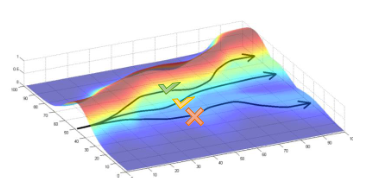
\includegraphics[scale=0.85]{ch3-rl/simulated-trajectories-levine-slides.png}
    \captionsetup{width=\textwidth} % set the width of the caption
    \caption{\textbf{Illustration of three simulated trajectories}, denoted as $\{\tau^{(i)}\}$ where $i=(1,2,3)$, traversing the parametric space $\theta\in\mathbb{R}^2$ under the policy $\pi_{\theta}$. Each trajectory is marked with a colored symbol (cross, check) representing its \textit{goodness} based on the reward function $R(\tau^{(i)})$. \textbf{Source:} \href{https://rail.eecs.berkeley.edu/deeprlcourse/}{Policy Gradients Lecture, Deep Reinforcement Learning Course} by Sergey Levine.}
    \label{fig:anatomy-rl-trajectories}
  \end{figure}
  
% algoritmo naive REINFORCE
\begin{algorithm}
    \caption{Vanilla Policy Gradient, aka REINFORCE}
    \begin{algorithmic}
    \STATE Initialize policy $\pi_{\theta}$, set learning rate $\alpha$
    % \STATE Generate $\tau=(s_0, a_0, ..., s_{T-1}, a_{T-1}, s_{T})$ by sampling from current $\pi_{\theta}$
    \FOR {$\text{iteration}=0, 1, 2, \dots, N$}
        \STATE Collect a set of trajectories $\mathcal{D}^{\pi_{\theta}}=\{\tau^{(i)}\}$ by sampling from the current policy $\pi_{\theta}$
        \STATE Calculate the returns $R(\tau)$ for each trajectory $\tau\in\mathcal{D^{\pi_{\theta}}}$
        \STATE Update the policy: $\theta \leftarrow \theta + \alpha \bigg(\frac{1}{\mid\mathcal{D^{\pi_{\theta}}}\mid}\sum_{\tau\in\mathcal{D}^{\pi_{\theta}}}\left[\sum_{t=0}^{T-1}\nabla_{\theta}\log\pi_{\theta}(a_{t}\mid s_{t})R(\tau)\right]\bigg)$
    \ENDFOR
    \end{algorithmic}
\end{algorithm}

\noindent The reward-to-go technique is a simple trick that can reduce the variance of the gradient estimator by taking advantage of the \textit{temporal structure} of the problem. The idea is to weight the gradient of the log-probability of an action $a_{t}$ by the sum of rewards from the current timestep $t$ to the end of the trajectory $T-1$. This way, the gradient of the log-probability of an action is only weighted by the consequence of that action on the future rewards, removing terms that don't depend on $a_{t}$. Let's introduce this technique by using the gradient estimation in Equation~\ref{eqn:reinforce-gradient-estimator} and replacing $R(\tau)$ naively using the sum of total trajectory reward\footnote{The same applies for discounted returns or other kind of returns $R(\tau)$.}.

\begin{equation}\label{eqn:reinforce-gradient-reward-to-go}
    \begin{split}
        \hat{g} &= \frac{1}{\mid\mathcal{D}^{\pi_{\theta}}\mid}\sum_{\tau\in\mathcal{D}^{\pi_{\theta}}}\left[\sum_{t=0}^{T-1} \nabla_{\theta} \log\pi_{\theta} (a_{t}\mid s_{t})\sum_{t=0}^{T-1} r_{t}\right] \\
        &= \frac{1}{\mid\mathcal{D}^{\pi_{\theta}}\mid}\sum_{\tau\in\mathcal{D}^{\pi_{\theta}}}\left[~\sum_{t=0}^{T-1} \nabla_{\theta} \log\pi_{\theta} (a_{t}\mid s_{t}) \bigg( \cancel{\sum_{t=0}^{t-1} r_{t}}  + \sum_{t'=t}^{T-1} r_{t'} \bigg)\right] \\
        &= \frac{1}{\mid\mathcal{D}^{\pi_{\theta}}\mid}\sum_{\tau\in\mathcal{D}^{\pi_{\theta}}}\left[~\sum_{t=0}^{T-1} \nabla_{\theta} \log\pi_{\theta} (a_{t}\mid s_{t}) \sum_{t'=t}^{T-1} r_{t'}\right] 
    \end{split}
\end{equation}

\noindent As we see at the end of Section~\ref{sec:gradient-estimation-score-function}, it is possible to reduce the variance of the gradient estimator by using a baseline function, $b(s_{t})$, without biasing the estimator. However, is the expectation of the score still unbiased in this setting? 

\begin{equation}\label{eqn:reinforce-gradient-estimator-baseline}
    \begin{split}
        \nabla_{\theta}\mathbb{E}_{\tau\sim p_{\theta}(\tau)} &= \mathbb{E}_{\tau\sim p_{\theta}(\tau)} \bigg[\sum_{t=0}^{T-1}\nabla_{\theta}\log\pi_{\theta}(a_{t}|s_{t})  \bigg(\sum_{t'=t}^{T-1} r_{t'}-b(s_{t'}) \bigg)\bigg]
    \end{split}
\end{equation}

\noindent The proof follows a similar argument as shown in Equation~\ref{eqn:score-function-expectation-zero}, with the key difference being that the expectation is taken with respect $p_{\theta}(\tau)$, which is a sequence of random variables. By leveraging the linearity of the expectation property, we can focus on a single term at step $t$ of Equation~\ref{eqn:reinforce-gradient-estimator-baseline} to demonstrate that the baseline does not affect the expectation of the score function. We split the trajectory sequence $\tau$ at step $t$ into: $\tau_{0:t}$ and $\tau_{t+1:T-1}$, and then expand it into state-action pairs\footnote{A criterion used when splitting the trajectory is that state-action pairs are formed given that $s_{t}$ is a consequence of action $a_{t-1}$, and taking action $a_{t}$ results in state $s_{t+1}$. Notice both expectations from step 1 and 2 in Equation~\ref{eqn:reinforce-baseline-unbiased}.}.

\begin{equation}\label{eqn:reinforce-baseline-unbiased}
   \begin{split}
        \mathbb{E}_{\tau\sim p_{\theta}(\tau)}\big[\nabla_{\theta}\log\pi_{\theta}(a_t|s_t) b(s_t) \big] &=  \mathbb{E}_{\tau_{(0:t)}}\big[\mathbb{E}_{\tau_{(t+1:T-1)}}[ \nabla_{\theta}\log \pi_{\theta}(a_{t}|s_{t})b(s_{t})]\big]  \\
        &= \mathbb{E}_{s_{0:t}, a_{0:t-1}}\big[\mathbb{E}_{s_{t+1:T}, a_{t:T-1}}[ \nabla_{\theta}\log \pi_{\theta}(a_{t}|s_{t})b(s_{t})]\big] \\
        &= \mathbb{E}_{s_{0:t}, a_{0:t-1}}\big[b(s_{t})\mathbb{E}_{s_{t+1:T}, a_{t:T-1}}[ \nabla_{\theta}\log \pi_{\theta}(a_{t}|s_{t})]\big] \\
        &= \mathbb{E}_{s_{0:t}, a_{0:t-1}}\big[b(s_{t})\mathbb{E}_{a_{t}}[ \nabla_{\theta}\log \pi_{\theta}(a_{t}|s_{t})]\big] \\
        &= \mathbb{E}_{s_{0:t}, a_{0:t-1}}\big[b(s_{t})\nabla_{\theta}\mathbb{E}_{a_{t}}[\log \pi_{\theta}(a_{t}|s_{t})]\big] \\
        &= \mathbb{E}_{s_{0:t}, a_{0:t-1}}\big[b(s_{t})\nabla_{\theta}1\big] \\
        &= 0
   \end{split}
\end{equation}

\noindent We can remove irrelevant variables from the expectation over the portion of the trajectory $\tau_{(t+1):(T-1)}$ because we are focusing on the term at step $t$. The only relevant variable is $a_{t}$, and the expectation $\mathbb{E}_{a_{t}}\log\pi_{\theta}(a_{t}\mid s_{t})$ is 1. Given that the
gradient with respect to $\theta$ of a constant is zero, and $b(s_{t})$ is multiplying it, the effect of the baseline on the expectation is nullified. This argument can be applied to any other term in the sequence due to the linearity of the expectation. Therefore, we have proven that using a baseline also keeps the gradient estimator unbiased in the policy gradient setting. \\

\noindent Choosing an appropriate baseline is a critical decision in reinforcement learning \citep{foundations-deeprl-series-l3}, as different methods can offer unique strengths and limitations. Common baselines include fixed values, moving averages, and learned value functions.

\begin{enumerate}
    \item Constant baseline: $b=\mathbb{E}\left[ R(\tau)\right]\approx \frac{1}{m}\sum_{i=1}^{m} R(\tau^{(i)})$
    \item Optimal constant baseline: $b=\frac{\sum_{i}(\nabla_{\theta} \log P_{\theta}(\tau^{(i)}))^{2} R(\tau^{(i)})}{\sum_{i}(\nabla_{\theta}\log P_{\theta}(\tau^{(i)}))^{2}}$ 
    \item Time-dependent baseline: $b_{t}=\frac{1}{m} \sum_{i=1}^{m} \sum_{k=t}^{T-1} R(s_{k}^{(i)}, a_{k}^{(i)})$ 
    \item State-dependent expected return: $b(s_{t}) = \mathbb{E}\left[r_{t} + r_{t+1} + r_{t+2} + \dots + r_{T-1}\right] = V^{\pi}(s_{t})$
\end{enumerate}


\noindent The control variates method can significantly reduce estimator variance, enhancing the stability and performance of RL algorithms \cite{NIPS2001_584b98aa}. Despite the nuances and differences among baseline methods, the primary concept is the \textit{advantage}, shown in Equation~\ref{eqn:pg-objective-with-value-baseline}, which refers to increase log probabilities of action $a_{t}$ proportionally to how much its returns, $r_{t}$, are better than the expected return under the current policy, which is determined by the value function $V^{\pi}(s_{t})$.

\begin{equation}\label{eqn:pg-objective-with-value-baseline}
    \mathbb{E}_{\tau\sim p_{\theta}(\tau)} \bigg[\sum_{t=0}^{T-1}\nabla_{\theta}\log\pi_{\theta}(a_{t}|s_{t}) \bigg(\underbrace{\sum_{t'=t}^{T-1} R(a_{t'}, s_{t'}) -V^{\pi}(s_{t})}_{\text{advantage}} \bigg) \bigg]
\end{equation}

\noindent What remains is how do we get estimates for $V^{\pi}$ in practice.

\section{Actor-Critic Methods}

Actor-Critic referred to learn concurrently models for the policy and the value function. This methods are more data efficient because they amortize the samples collected $\mathcal{D}^{\pi_{\theta}}$ used for Monte Carlo estimations while reducing the variance of the gradient estimator. The actor controls how the agent behaves---\textit{by updating the policy parameters $\theta$ as we see in previous sections}---whereas the critic measures how good the taken action is, and could be a state-value ($V$) or action-value ($Q$)\footnote{Action-value function ($Q$) refers to the value of take action $a$ on state $s$ under a policy $\pi$.} function. Notice that we are combining in some way both approaches for solving MDPs as is depicted in Figure~\ref{fig:rl-model-free-taxonomy}.\\

\noindent We are introducing a new function approximator for the value function, $V_{\phi}(s_{t})$, where $\phi$ are the parameters of the value function. 

\begin{equation}\label{eqn:actor-critic-objective}
    \mathbb{E}_{\tau\sim p_{\theta}(\tau)} \bigg[\sum_{t=0}^{T-1}\nabla_{\theta}\log\pi_{\theta}(a_{t}|s_{t}) \bigg( \sum_{t'=t}^{T-1} R(a_{t'}, s_{t'}) - V_{\phi}^{\pi}(s_{t}) \bigg) \bigg]
\end{equation}

\noindent The objective is to minimize the mean squared error (MSE) between the estimated value and the empirical return, i.e. we are regress the value against empirical return in a supervised learning fashion. 
% \ca{Mencionar conexión con el mse a partir de la varianza del gradiente? (Seita post)}:

\begin{equation}\label{eqn:value-function-loss}
   \phi \leftarrow \underset{\phi}{\arg\min} \frac{1}{\mid\mathcal{D}^{\pi_{\theta}}\mid}\sum_{\tau\in\mathcal{D}^{\pi_{\theta}}}\sum_{t=0}^{T-1}\left[\left(\left(\sum_{t'=t}^{T-1} R(a_{t'}, s_{t'})\right) - V_{\phi}(s_{t})\right)^2~\right]
\end{equation}

\noindent Algorithm~4 describes the steps for a REINFORCE variant with advantage , which combines the actor-critic approach with the traditioinoal REINFORCE algorithm. More components were introduced and can influence in the performance when the algorithm is implemented. For instance, the policy and value networks can share parameters or not. A useful study that make abalations and suggestions to pay attention when these algorithms are implemented is \textit{What Matters In On-Policy Reinforcement Learning? A Large-Scale Empirical Study (Andrychowicz, 2020 \cite{andrychowicz2020mattersonpolicyreinforcementlearning})}.\\

\begin{algorithm}
    \caption{REINFORCE with advantage}
    \begin{algorithmic}
    \STATE Initialize policy $\pi_{\theta}$
    \STATE Initialize value $V_{\phi}$
    \STATE Set learning rates $\alpha_{a}$ and $\alpha_{c}$
    \FOR {$\text{iteration}=0, 1, 2, \dots, N$}
        \STATE Collect a set of trajectories $\mathcal{D}^{\pi_{\theta}}=\{\tau^{(i)}\}$ by sampling from the current policy $\pi_{\theta}$
        \STATE Calculate the returns $R(\tau)$ for each trajectory $\tau\in\mathcal{D}^{\pi_{\theta}}$
        \STATE Update the policy:
        \STATE \qquad$\theta \leftarrow \theta + \alpha_{a} \left(\frac{1}{\mid\mathcal{D^{\pi_{\theta}}}\mid}\sum_{\tau\in\mathcal{D}^{\pi_{\theta}}}\left[\sum_{t=0}^{T-1}\nabla_{\theta}\log\pi_{\theta}(a_{t}\mid s_{t})\left(\sum_{t'=t}^{T-1} R(a_{t'}, s_{t'}) - V_{\phi}^{\pi_{\theta}}(s_{t})\right)\right]\right)$
        \STATE Update the value:
        \STATE \qquad $\phi \leftarrow \phi + \alpha_{c} \left(\frac{1}{\mid\mathcal{D}^{\pi_{\theta}}\mid}\sum_{\tau\in\mathcal{D}^{\pi_{\theta}}}\left[\sum_{t=0}^{T-1}\left(\sum_{t'=t}^{T-1} R(a_{t'}, s_{t'}) - V_{\phi}^{\pi_{\theta}}(s_{t})\right)\nabla_{\phi}V_{\phi}^{\pi_{\theta}}(s_{t})\right]\right)$
    \ENDFOR
    \end{algorithmic}
\end{algorithm}

% \noindent \textbf{Advantage estimation}. Variance reduction by discounting, treateing $\gamma$ as an hyperparameter to improve $Q$ estimate...then A3C with Q k-steps lookahead estimation, and finally GAE. \ca{TODO...}


\section{Improving Sample Efficiency: Behavior and Target Policies}

% \ca{Util de referencia en literatura \cite{peshkin2002learning}}

The main drawback of the REINFORCE algorithm is its sample complexity. Once we roll out the policy and collect the data, we cannot reuse it after the policy has been updated. We must collect new data following the \textit{target policy} $\pi_{\theta}$ that we want to update. In RL literature, this is referred to as \textit{on-policy} learning. Reusing the data $\mathcal{D}\sim\pi_{\theta_{\text{old}}}$ to update the current policy $\pi_{\theta}$ would significantly improve sample efficiency\footnote{This issue also arises when attempting to transfer behavior from one task to another using existing data.}. However, once we update the policy, the previously collected data is no longer valid because the policy has changed. The distribution from which the data was sampled is now $\pi_{\theta_{\text{old}}}$. \\

\noindent Using behavior data learned from another policy, known as a \textit{behavior policy}, to update the current policy is referred to as \textit{off-policy} learning in RL literature. Let's introduce a \textit{behavior policy} in the RL objective defined in Equation~\ref{eqn:rl-objective} using \href{https://timvieira.github.io/blog/post/2014/12/21/importance-sampling/}{importance sampling} (See Mckay book, Section 29.2 \cite{mackay-book}):

% Derive RL objective with importance sampling to use data from another policy
\begin{equation}\label{eqn:derive-rl-objective-with-is}
    \begin{split}
        \nabla_{\theta}\mathcal{J}(\theta) &= \mathbb{E}_{\tau \sim p_{\theta}(\tau)}\bigg[ \nabla_{\theta}\log p_{\theta}(\tau) R(\tau)\bigg] \\
        &= \mathbb{E}_{\tau \sim p_{\theta}(\tau)} \bigg[ \frac{\nabla_{\theta}p_{\theta}(\tau)}{p_{\theta}(\tau)} R(\tau) \bigg] \\
        &= \int_{\mathcal{X}} p_{\theta}(\tau) \frac{\nabla_{\theta}p_{\theta}(\tau)}{p_{\theta}(\tau)} R(\tau) d\tau \\
        &= \int_{\mathcal{X}} \frac{p_{\theta_{\text{old}}}(\tau)}{p_{\theta_{\text{old}}}(\tau)} \cancel{p_{\theta}(\tau)} \frac{\nabla_{\theta}p_{\theta}(\tau)}{\cancel{p_{\theta}}(\tau)} R(\tau) d\tau \\
        &= \int_{\mathcal{X}} p_{\theta_{\text{old}}}(\tau) \frac{\nabla_{\theta}p_{\theta}(\tau)}{p_{\theta_{\text{old}}}(\tau)} R(\tau) d\tau \\
        &= \mathbb{E}_{\tau\sim p_{\theta_{\text{old}}}(\tau)} \bigg[\frac{\nabla_{\theta} p_{\theta}(\tau)}{p_{\theta_{\text{old}}}(\tau)} R(\tau)\bigg]
    \end{split}
\end{equation}

\noindent We derive a new objective that is more general and reconciles both \textit{on-policy} and \textit{off-policy} learning in the importance weight,
or importance correction ($p_{\theta}(\tau) / p_{\theta_{\text{old}}}(\tau)$). 

% RL objective with IS
\begin{equation}\label{eqn:rl-objective-with-is}
    \mathcal{J}_{\text{IS}}(\theta) = \mathbb{E}_{\tau\sim p_{\theta_{\text{old}}}(\tau)}\bigg[\frac{p_{\theta}(\tau)}{p_{\theta_{\text{old}}}(\tau)} R(\tau)\bigg]
\end{equation}

\noindent We can assume that the data collected from the behavior policy is
not so different from the target policy, and use first order approximation to
update the policy. 

\begin{equation}\label{eqn:rl-objective-is-linear-aprox}
    \begin{split}
        \nabla_{\theta}\mathcal{J}(\theta)\rvert_{\theta=\theta_{\text{old}}} &= \mathbb{E}_{\tau\sim p_{\theta_{\text{old}}}(\tau)} \bigg[\frac{\nabla_{\theta} p_{\theta}(\tau)\rvert_{\theta=\theta_{\text{old}}}}{p_{\theta_{\text{old}}}(\tau)} R(\tau)\bigg] \\
        &= \mathbb{E}_{\tau\sim p_{\theta_{\text{old}}}(\tau)} \big[\nabla_{\theta}\log p_{\theta}(\tau)\rvert_{\theta=\theta_{\text{old}}} R(\tau) \big]
    \end{split}
\end{equation}


\noindent \textbf{The problem with first order approximation}. The gradient estimation it is good only in the inmediate vecinity, because is a local approximation of the function. Hence, the step size is crucial to avoid a policy degradation, a situation where the policy is updated with a bad gradient,
it is difficult to recover from this situation. Given that the data is collected by the policy, the feedback loop can be dangerous for the training
stability. \\

\section{Trust Region and Proximal Policy Optimization}\label{sec:trpo-ppo}

Trust Region Policy Optimization (TRPO) \cite{schulman2015trust} allows us to
avoid the policy degradation given bad updates. The idea is to 
define a trust region in which update the policy parameter is safer and
balancing the policy improvement with stability.

\begin{align}
    \text{Surrogate loss:} \quad & \underset{\pi_{\theta}}{\max}~L(\pi) = \mathbb{E}_{\pi_{\theta_{\text{old}}}} \left[ \frac{\pi_{\theta}(a\mid s)}{\pi_{\theta_{\text{old}}}(a\mid s)} A^{\pi_{\theta_{\text{old}}}}(s, a) \right] \label{eqn:trpo-loss} \\
    \text{Constraint:} \quad & \mathbb{E}_{\pi_{\text{old}}} \left[ D_{\text{KL}}(\pi_{\theta} || \pi_{\theta_{\text{old}}}) \right]  \leq \epsilon, \nonumber
\end{align}

%\noindent \textbf{Maximize data efficiency in comparison to traditional policy gradients}. 

\noindent Increase data efficiency while avoiding step size problems in updating parameters, compared to traditional policy gradients (PG). The main idea is to improve a surrogate objective significantly while making minimal changes to the policy. These minimal changes are quantified using the KL divergence between action distributions. The trust region is the area where the new policy remains close to the old one, guarantee training stability. \\

% The trust region is the area where the new policy remains close to the old one, allowing for constrained improvement. \\

\noindent Proximal Policy Optimization (PPO) \cite{schulman2017proximal} is about simplify TRPO in order to (i) be easier to implement avoiding solve the second order optimization in Equation~\ref{eqn:trpo-loss}, (ii) taking advantage of first order optimizer such as ADAM \cite{kingma2017adammethodstochasticoptimization}, and (iii) be more compatible with neural networks operations such as dropout that are incompatible with TRPO setting. \\

\noindent Let's rename the importance weights as the probability ratio $r$: 

\begin{equation}\label{eqn:importance-ratio-is}
    r_{t}(\theta) = \frac{\pi_{\theta}(a_{t}\mid s_{t})}{\pi_{\theta_{\text{old}}}(a_{t}\mid s_{t})}
\end{equation}

\noindent The strategy is to keep this ratio closer to 1. We can create a trust region via clipping the ratio to force within a range $\left[1-\epsilon, 1+\epsilon \right]$. 

\begin{equation}\label{eqn:clip-ac-objective}
\mathcal{L}^{\text{CLIP}}(\theta) = \hat{\mathbb{E}}_t \left[ \min \left( r_t(\theta) \hat{A}_t, \text{clip}(r_t(\theta), 1 - \epsilon, 1 + \epsilon) \hat{A}_t \right) \right]
\end{equation}

\noindent For a walkthrough implementation that cover important details avoid in the paper and that impact significatnly in the performance, review the work \textit{``The 37 implementation details of proximal policy optimization''} (Huang, 2023 \cite{dlr191986}).


% algoritmo naive REINFORCE
\begin{algorithm}
    \caption{Proximal Policy Optimization (PPO), Actor-Critic Style}
    \begin{algorithmic}
    \STATE Initialize policy parameter $\theta$, set learning rate $\alpha$
    \STATE Initialize value $V_{\phi}$
    \FOR{$\text{iteration}=0, 1, 2, \dots N$}
        \FOR{$\text{actor}=0, 1, 2, \dots M$}
            \STATE Run policy $\pi_{\theta_{\text{old}}}$ in environment for $T$ timesteps        
            \STATE Compute advantage estimates $\hat{A}_{0}, \dots, \hat{A}_{T-1}$
        \ENDFOR
        \STATE Optimize surrogate $\mathcal{L}^{\text{CLIP}}$ wrt $\theta$ (Equation~\ref{eqn:clip-ac-objective}), with $K$ epochs and minibatch size $M\leq NT$
    \ENDFOR
    \end{algorithmic}
\end{algorithm}


\section{Reinforcement Learning From Human Feedback}\label{sec:rlhf}

Reinforcement learning from human feedback (RLHF) is introducing the human within the reinforcement loop, providing the agent the necessary feedback to learn the intended behavior. The idea is learning a reward model that capture the behavior from humans, and use the model to provide the feedback in asynchrounous way, which means that during agent training it is not require to wait the human for a respond with the reward\footnote{A static reward model is equivalent to extract information in a off-policy fashion. But, the reward model can update dynamically with the agent, taking new information from the on-policy trajectoriesa.}; making fully compatible and scalable in the model-free and online learning setting studied in this chapter. \\

\noindent A reward function elicit changes in the system behavior, that is the whole point of reinforcement learning. By trial-and-error, figuring out what is the best behavior that maximize the reward, and by that means, the intended goal. However, the reward function is a key component in the RL setting and is not always easy to design it. Outside video games with clear rules and scenarios, real world is highly complex, erratic, and dificult to simulate. Therefore, more than sometimes align the intended behavior with the reward function is a difficult task. Beyond the realm of RL, use human feedback in this setting provide a useful way to align matching distribution learning systems with the human preferences. Perhaps, the most significant example is in large language models, in which RLHF can mute the behavior of an inherent autocompletion system into a more instructional and conversationl behavior \cite{ouyang2022training}.

\begin{figure}[ht]
    \centering
    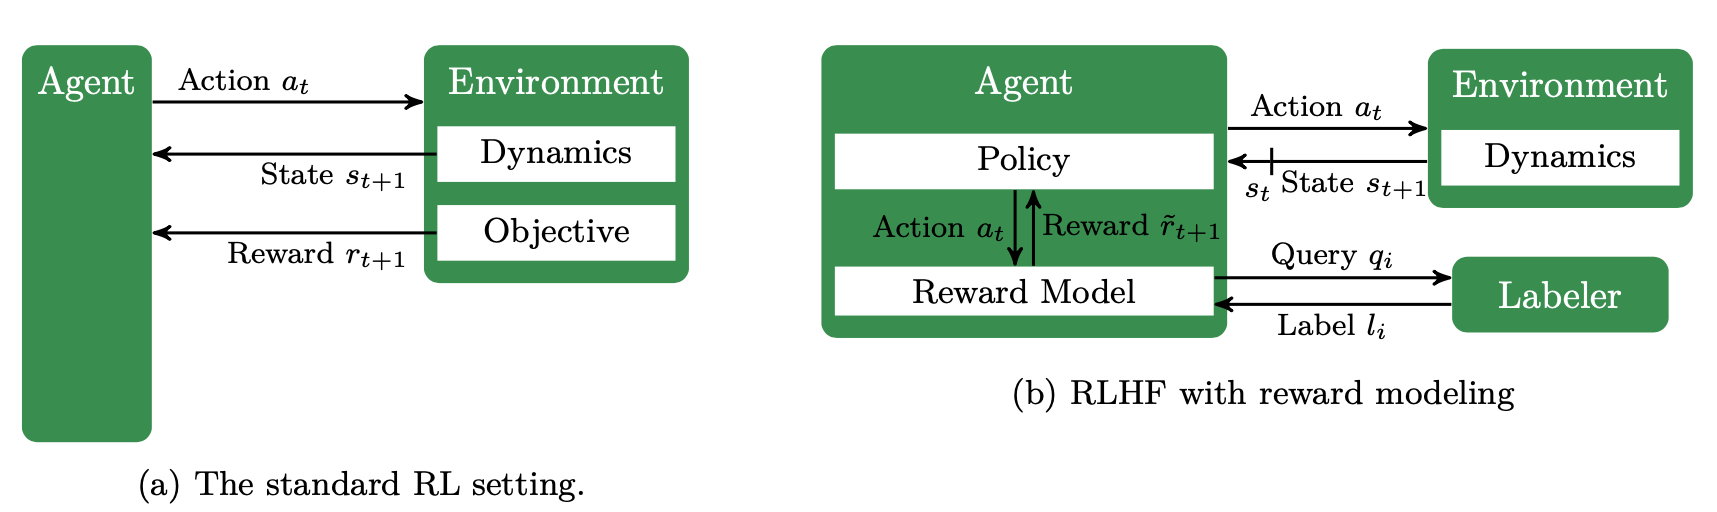
\includegraphics[scale=0.55]{ch3-rl/rl-standard-vs-rlhf-settings.png}
    \captionsetup{width=\textwidth} % set the width of the caption
    \caption{\textbf{Left:} A standard RL settings. \textbf{Right:} A RLHF setting considering reward modeling. \textbf{Source:} \href{https://arxiv.org/abs/2312.14925}{A Survey of Reinforcement Learning from Human Feedback (Kaufmann et al., 2024) \cite{kaufmann2023survey}}. Notice how the reward model is decoupled from the environment and the relation highlighted between the reward model and an oracle (i.e. labeler) who provides a label to a given query.}
    \label{fig:rlhf-setting}
  \end{figure}

\noindent \textbf{Training the reward model}. Translate the human feedback 
from a collection of trajectory samples into a reward signal. However,
the human feedback can be noisy, inconsistent, and sparse. So, instead of
using the human feedback directly, it is used a reward model that learns
via an utility function that design to consume different types of feedbacks. For instance, a common setting is a binary comparison between trajectories where a utilify function is learned from the human preference between both using the Bradley-Terry model \cite{bradley-terry-model}. \\

\begin{equation*}
P(\tau_{1}\succ\tau_{2}) = \frac{1}{1 + \exp(R(\tau_{2}) - R(\tau_{1}))}
\end{equation*}

\noindent given a collection of trajectories $\mathcal{D}$ where $\succ$ means ``preferred to'' and $R(\tau)$ correponds to the utility (i.e. return in the context of RL) and it could be between an intermediate feature maps that allows to the human gives feedback in a useful way but provide a scalar signal easily to digest by the agent. The reward model can be trained using supervised learning, imitation learning, or inverse reinforcement learning. The reward model can be used in different ways, such as reward shaping, reward augmentation, or reward correction. \\

\begin{equation}
    \underset{\phi}{\max} \prod_{i=1}^{N}\frac{1}{1 + \exp\left(1 + \exp(R_{\Phi}) \right)}
\end{equation}

% \noindent \textbf{Alignment via reward modeling}. Train a reward model over human preferences \cite{leike2018scalable}, then use it to train the agent. The model can provide a reward signal that is more aligned with the human preferences. \\

\noindent Several human feedback types can distill into rewards models such as critique, comparisons, inter-temporal feedback, proxy rewards, social behavior, improvements, and natural language \cite{kaufmann2023survey}. Specifically,
for visual perception tasks, some interesting research lines are leveraging general human knowledge from large pretrained visual language models to provide feedback to the agent if it achieve success (i.e. success detectors) on the task in which is reinforced \cite{du2023visionlanguagemodelssuccessdetectors}. 
The main point is that once we have a reward model we can move from a standard RL setting to a RLHF setting, as shown in Figure~\ref{fig:rlhf-setting}. The
reward model requires a labeler to encode the human preferences into the
model weights, but once it is trained, the human preferences can be use asynchrounous and continuosly to provide feedback. \\

% In the context of diffusion models \cite{black2023training}, a language vision for the model (e.g. LLaVA) allows into a joint-embedding space and compute a BERT score. model (e.g. LLaVA) for prompt alignment. The idea is to give samples generated. There is also the work that \cite{lee2023aligning}.


\section{Summary}

In this chapter, we have explored the foundational concepts and methodologies in reinforcement learning (RL). The core of RL is the interaction between an agent and its environment, where learning occurs through trial-and-error. The agent's goal is to maximize cumulative rewards by taking actions based on its observations, influencing the state of the environment, and receiving rewards. \\

\noindent We began by introducing the Markov Decision Process (MDP), a mathematical framework that describes the interaction between the agent and the environment. An MDP is characterized by a state space, action space, transition probabilities, and reward functions. The agent aims to learn a policy that maximizes the expected return, which is the sum of discounted rewards over time. \\

\noindent We then delved into policy optimization methods, focusing on policy gradients, a popular approach in model-free RL. Policy gradient methods reduce RL to a problem of stochastic gradient descent, leveraging trajectories of state-action pairs to update the policy parameters. We discussed techniques such as the reward-to-go and baselines to reduce the variance of gradient estimators, thus improving learning efficiency. \\

\noindent Additionally, we examined how RL can be integrated with diffusion models to enhance sample generation. By training a reward model to align generated samples with desired goals, agents can learn to produce high-quality outputs in tasks such as image generation and other creative applications. \\

\noindent In conclusion, reinforcement learning offers a powerful framework for designing intelligent agents capable of learning optimal behaviors through interaction with their environment. By understanding and implementing the principles and techniques covered in this chapter, one can develop sophisticated RL agents for a wide range of applications \\